\section{Justificaci\'o del projecte}

\begin{figure}[!h]
	\centering
	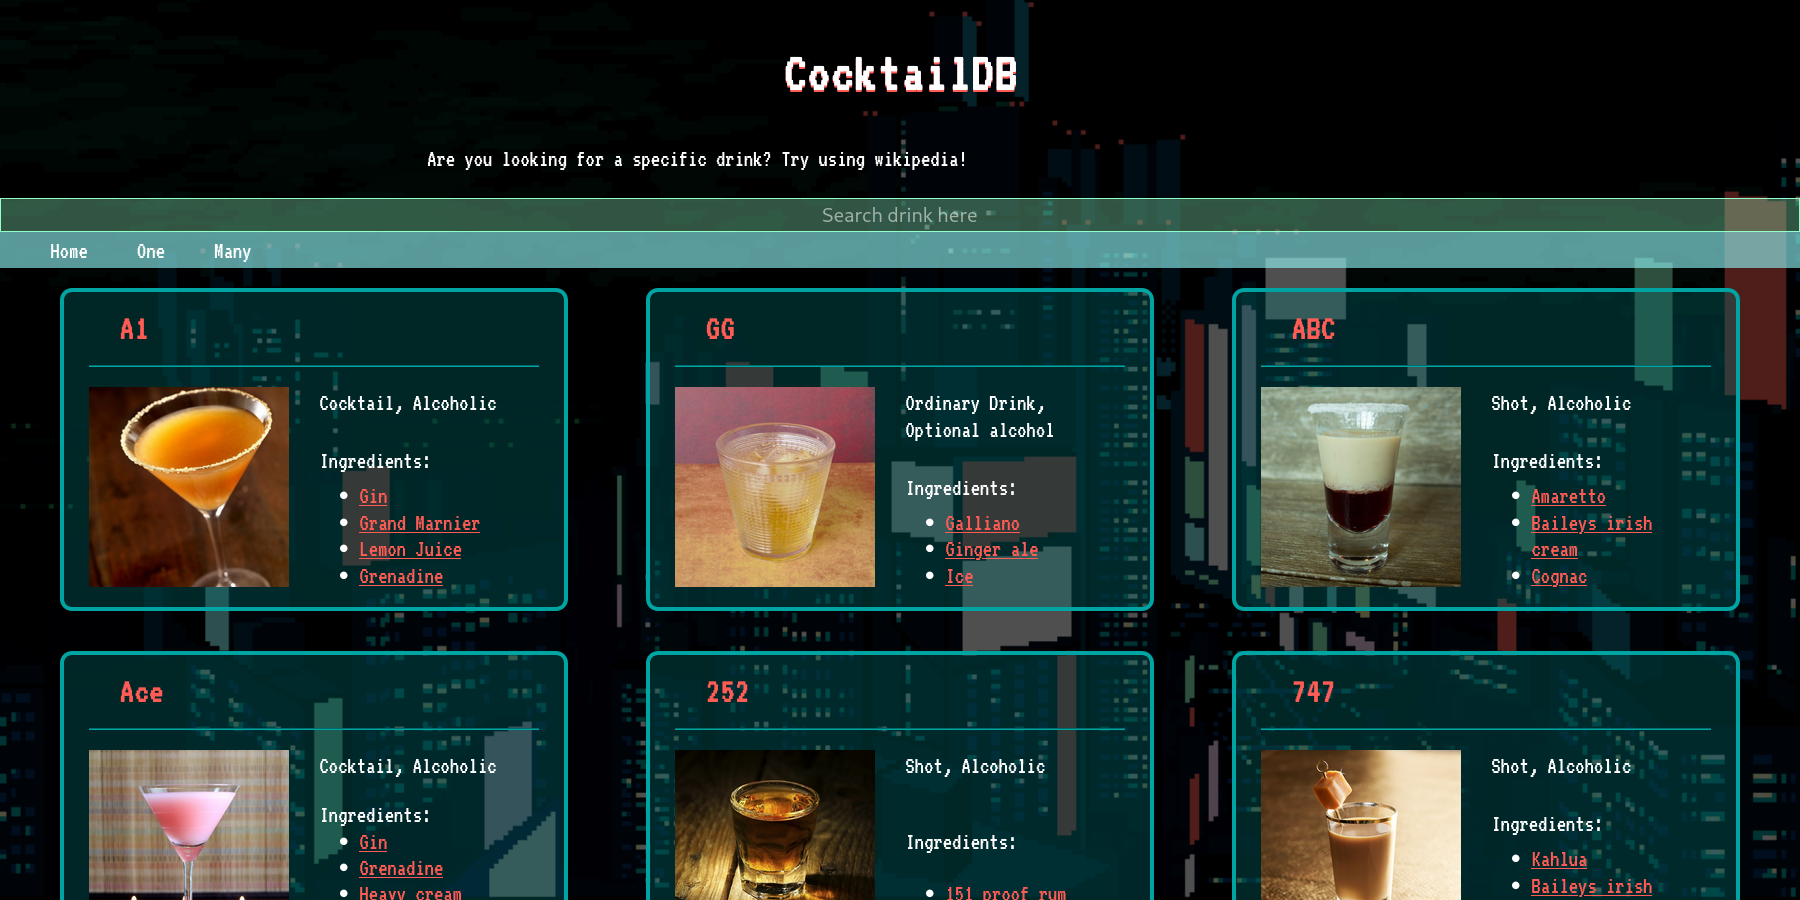
\includegraphics[width=0.8\columnwidth]{cocktailDB_example.png}
	\caption{Captura de la p\`agina}
\end{figure}

Per fer l'aplicaci\'o de l'api, hem utilitzat CocktailDB,
una api que d\'ona informaci\'o sobre cocktails.

CocktailDB \'es una api de lliure \'us que d\'ona informaci\'o sobre cocktails.
T\'e varies trucades \'utils per aconseguir informaci\'o de la base de dades,
que \'es enviada en forma de llista, a on cada atribut \'es un cocktail diferent.

Una altra ra\'o per la qual hem decidit utilitzar aquesta api en concret
\'es que \'es de lliure \'us.
Aix\`o vol dir que no t\'e un rate limit aparent,
per la qual cosa no ens hem de precupar pel l\'imit de trucades a l'api,
i tampoc ens hem de registrar per utilitzar-la.
CocktailDB tampoc necessita registrar-se per utilitazar-la,
la qual cosa facilita el treball.

\begin{figure}[!h]
	\centering
	\includegraphics[width=0.6\columnwidth]{cocktaildb.png}
	\caption{P\`agina principal de cocktaildb}
\end{figure}

L'estil de la web est\`a basat en l'ambientaci\'o de Va-11 Hall-a,
una nove\lgem a visual on la principal mec\`anica \'es preparar cocktails.
Els colors de la p\`agina i la lletra estan fets de tal manera
que encaixin amb l'est\`etica del fons,
que est\`a tret de la novela visual.

\begin{figure}[!h]
	\centering
	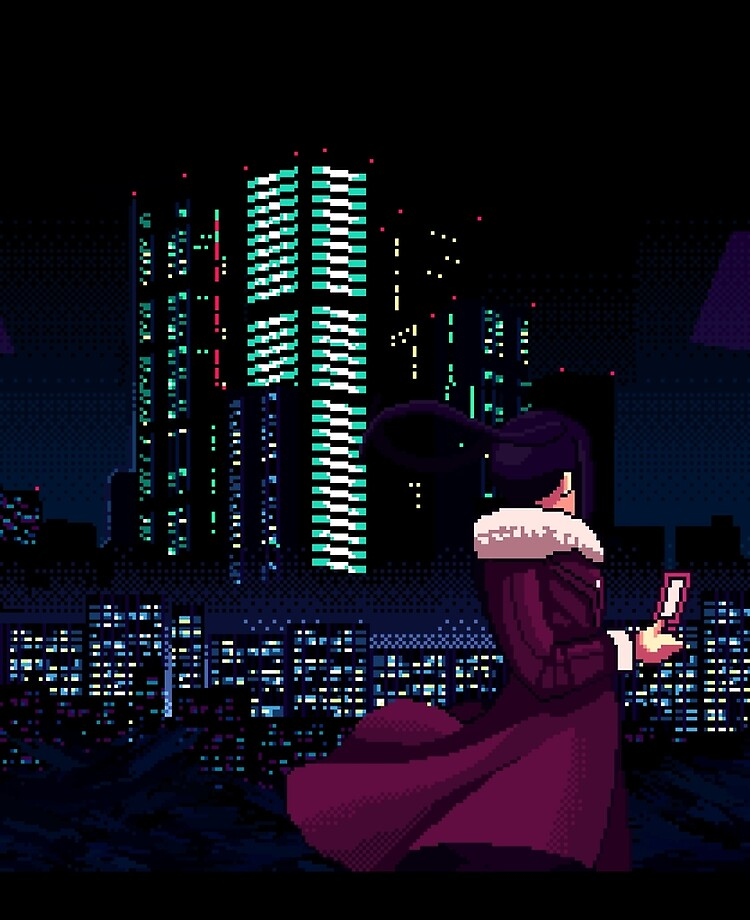
\includegraphics[width=0.3\columnwidth]{va-11 hall-a.jpg}
	\caption{Portada de Va-11 Hall-a}
\end{figure}

Per fer l'estil de la p\`agina no s'ha utilitzat cap template d'html,
hem preferit fer el treball nosaltres en comptes de copiar i enganxar d'internet.
